\documentclass[UTF8, a4paper, 11pt]{article}
\usepackage{diagbox}
\usepackage{subfigure}
\usepackage[UTF8, scheme=plain]{ctex}
\usepackage{fontspec}
\usepackage{float}
\usepackage{amsmath}
\newtheorem{myDef}{Definition}
\usepackage{graphicx}
\usepackage{geometry}
\usepackage{listings}
\usepackage{xcolor}
\usepackage{caption}
\geometry{scale=0.8}
\linespread{1.5}
\usepackage{hyperref}
\usepackage{color}
\usepackage{fontspec}
\usepackage{enumitem}
\usepackage[linesnumbered,boxed]{algorithm2e}    
\usepackage{xeCJK}
\usepackage{indentfirst} 
\graphicspath{{Pics/}} 	% 在于.tex同级的目录下创建名为pic的文件夹,存放图片


\setlength{\parindent}{2em}

\lstset{
    language={C},
    frame=shadowbox,
    breaklines=true,
    numbers=left,
    backgroundcolor=\color[RGB]{245,245,244},
    rulesepcolor=\color{red!20!green!20!blue!20},
    numberstyle={\color[RGB]{0,192,192}\tiny},
    basicstyle=\footnotesize \fontspec{Source Code Pro}
}
\setenumerate[1]{itemsep=0pt,partopsep=0pt,parsep=\parskip,topsep=0pt}
\setitemize[1]{itemsep=0pt,partopsep=0pt,parsep=\parskip,topsep=0pt}
\setdescription{itemsep=0pt,partopsep=0pt,parsep=\parskip,topsep=0pt}


\title{	
\normalfont \normalsize
\textsc{School of Data and Computer Science, Sun Yat-sen University} \\ [25pt] %textsc small capital letters
\rule{\textwidth}{0.5pt} \\[0.4cm] % Thin top horizontal rule
\huge 数电实验6\\ % The assignment title
\rule{\textwidth}{2pt} \\[0.5cm] % Thick bottom horizontal rule
\author{18308045 谷正阳}
\date{\normalsize\today}
}

\begin{document}
\maketitle
\tableofcontents
\newpage
\section{仿真实验}
\subsection{八选一数据选择器}
\subsubsection{二选一数据选择器卡诺图}
\begin{table}[H]
\begin{tabular}{|l|l|l|}
\hline
\diagbox{l0l1}{S0} & 0 & 1 \\ \hline
00                 & 0 & 0 \\ \hline
01                 & 0 & 1 \\ \hline
11                 & 1 & 1 \\ \hline
10                 & 1 & 0 \\ \hline
\end{tabular}
\end{table}
\subsubsection{子电路图}
每个二选一数据选择器可看作是一个2层的二叉树,用7个二选一数据选择器,构成一个4层的满二叉树,共有8个叶子节点。
\begin{figure}[H]
    \centering
    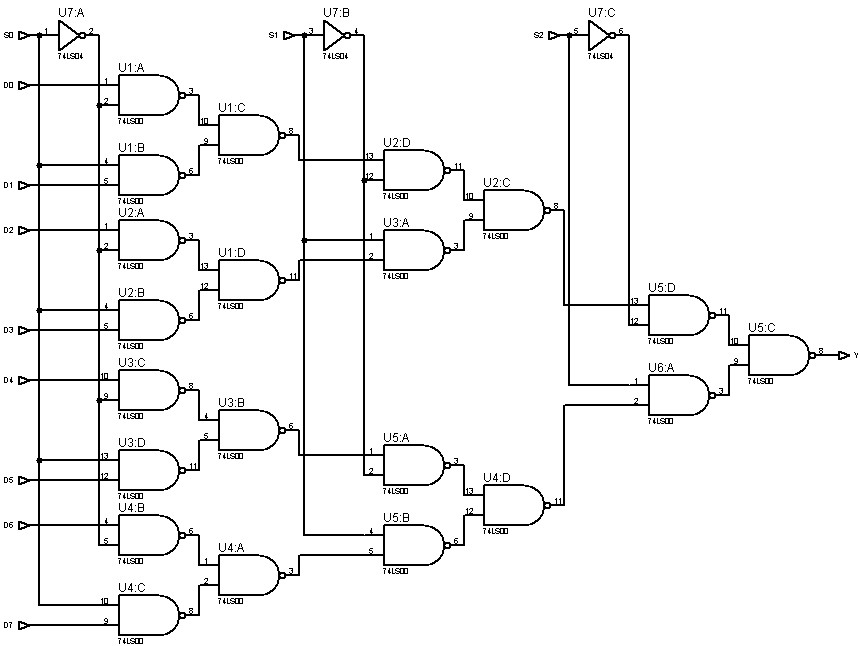
\includegraphics[width=0.8\textwidth]{ex6.1电路图2.jpg}
\end{figure}
\subsubsection{电路图}
D0-D7以分别接00011110,S0-S7分别接Q1-Q3。
\begin{figure}[H]
    \centering
    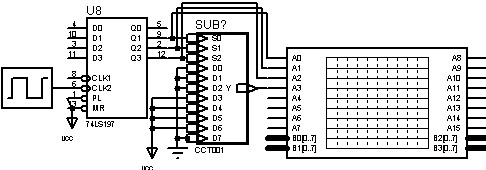
\includegraphics[width=0.8\textwidth]{ex6.1电路图1.jpg}
\end{figure}
\subsubsection{波形图}
\begin{figure}[H]
    \centering
    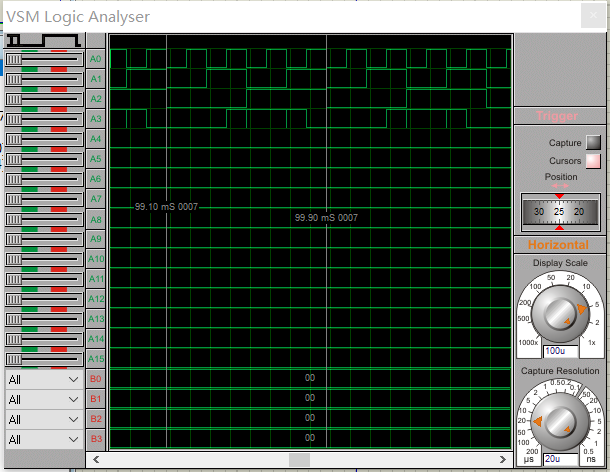
\includegraphics[width=0.8\textwidth]{ex6.1波形图.png}
\end{figure}
\subsection{AU}
\subsubsection{电路图}
加法和减法的输出均有:
$$Y=A\oplus B$$
,进位/错位列真值表用ABS进行选择。
\begin{figure}[H]
    \centering
    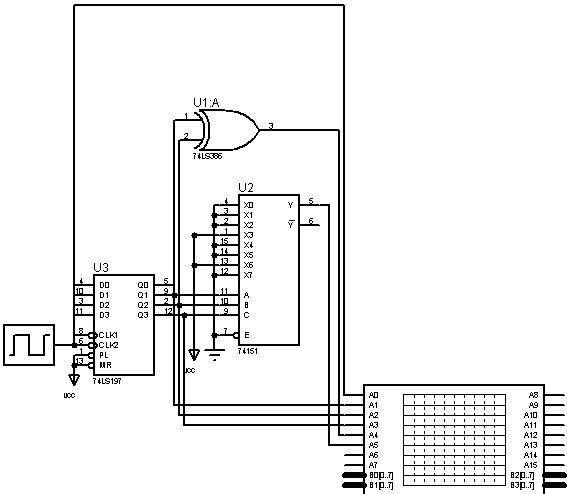
\includegraphics[width=0.8\textwidth]{ex6.2电路图.jpg}
\end{figure}
\subsubsection{波形图}
A0为时钟信号,A1、A2、A3分别为A、B、S,A4、A5分别为Y、Cn。
\begin{figure}[H]
    \centering
    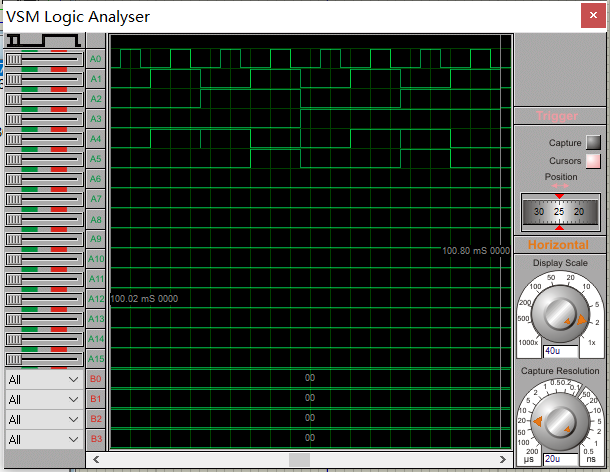
\includegraphics[width=0.8\textwidth]{ex6.2波形图.png}
\end{figure}
\subsection{LU}
\subsubsection{电路图}
\begin{figure}[H]
    \centering
    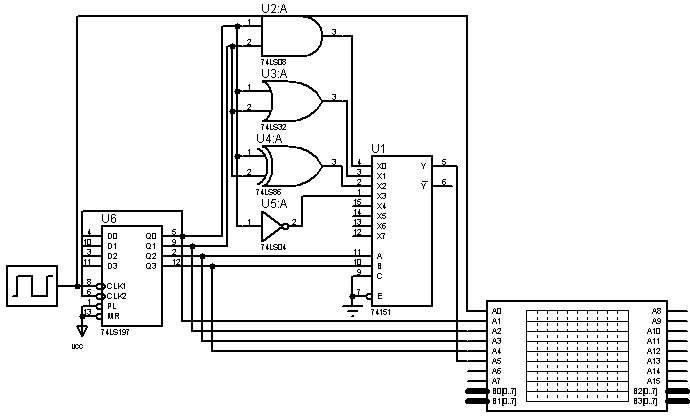
\includegraphics[width=0.8\textwidth]{ex6.3电路图.jpg}
\end{figure}
\subsubsection{波形图}
A0、A1、A2、A3、A4、A5分别为CP、A、B、S0、S1、Y。
\begin{figure}[H]
    \centering
    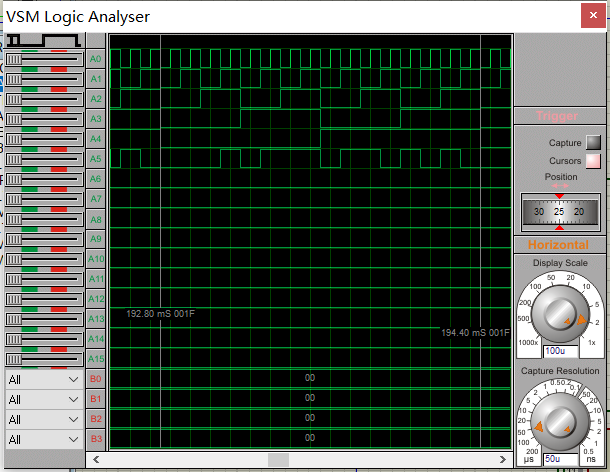
\includegraphics[width=0.8\textwidth]{ex6.3波形图.png}
\end{figure}
\section{实验箱实验}
\subsection{AU}
\begin{figure}[H]
    \centering
    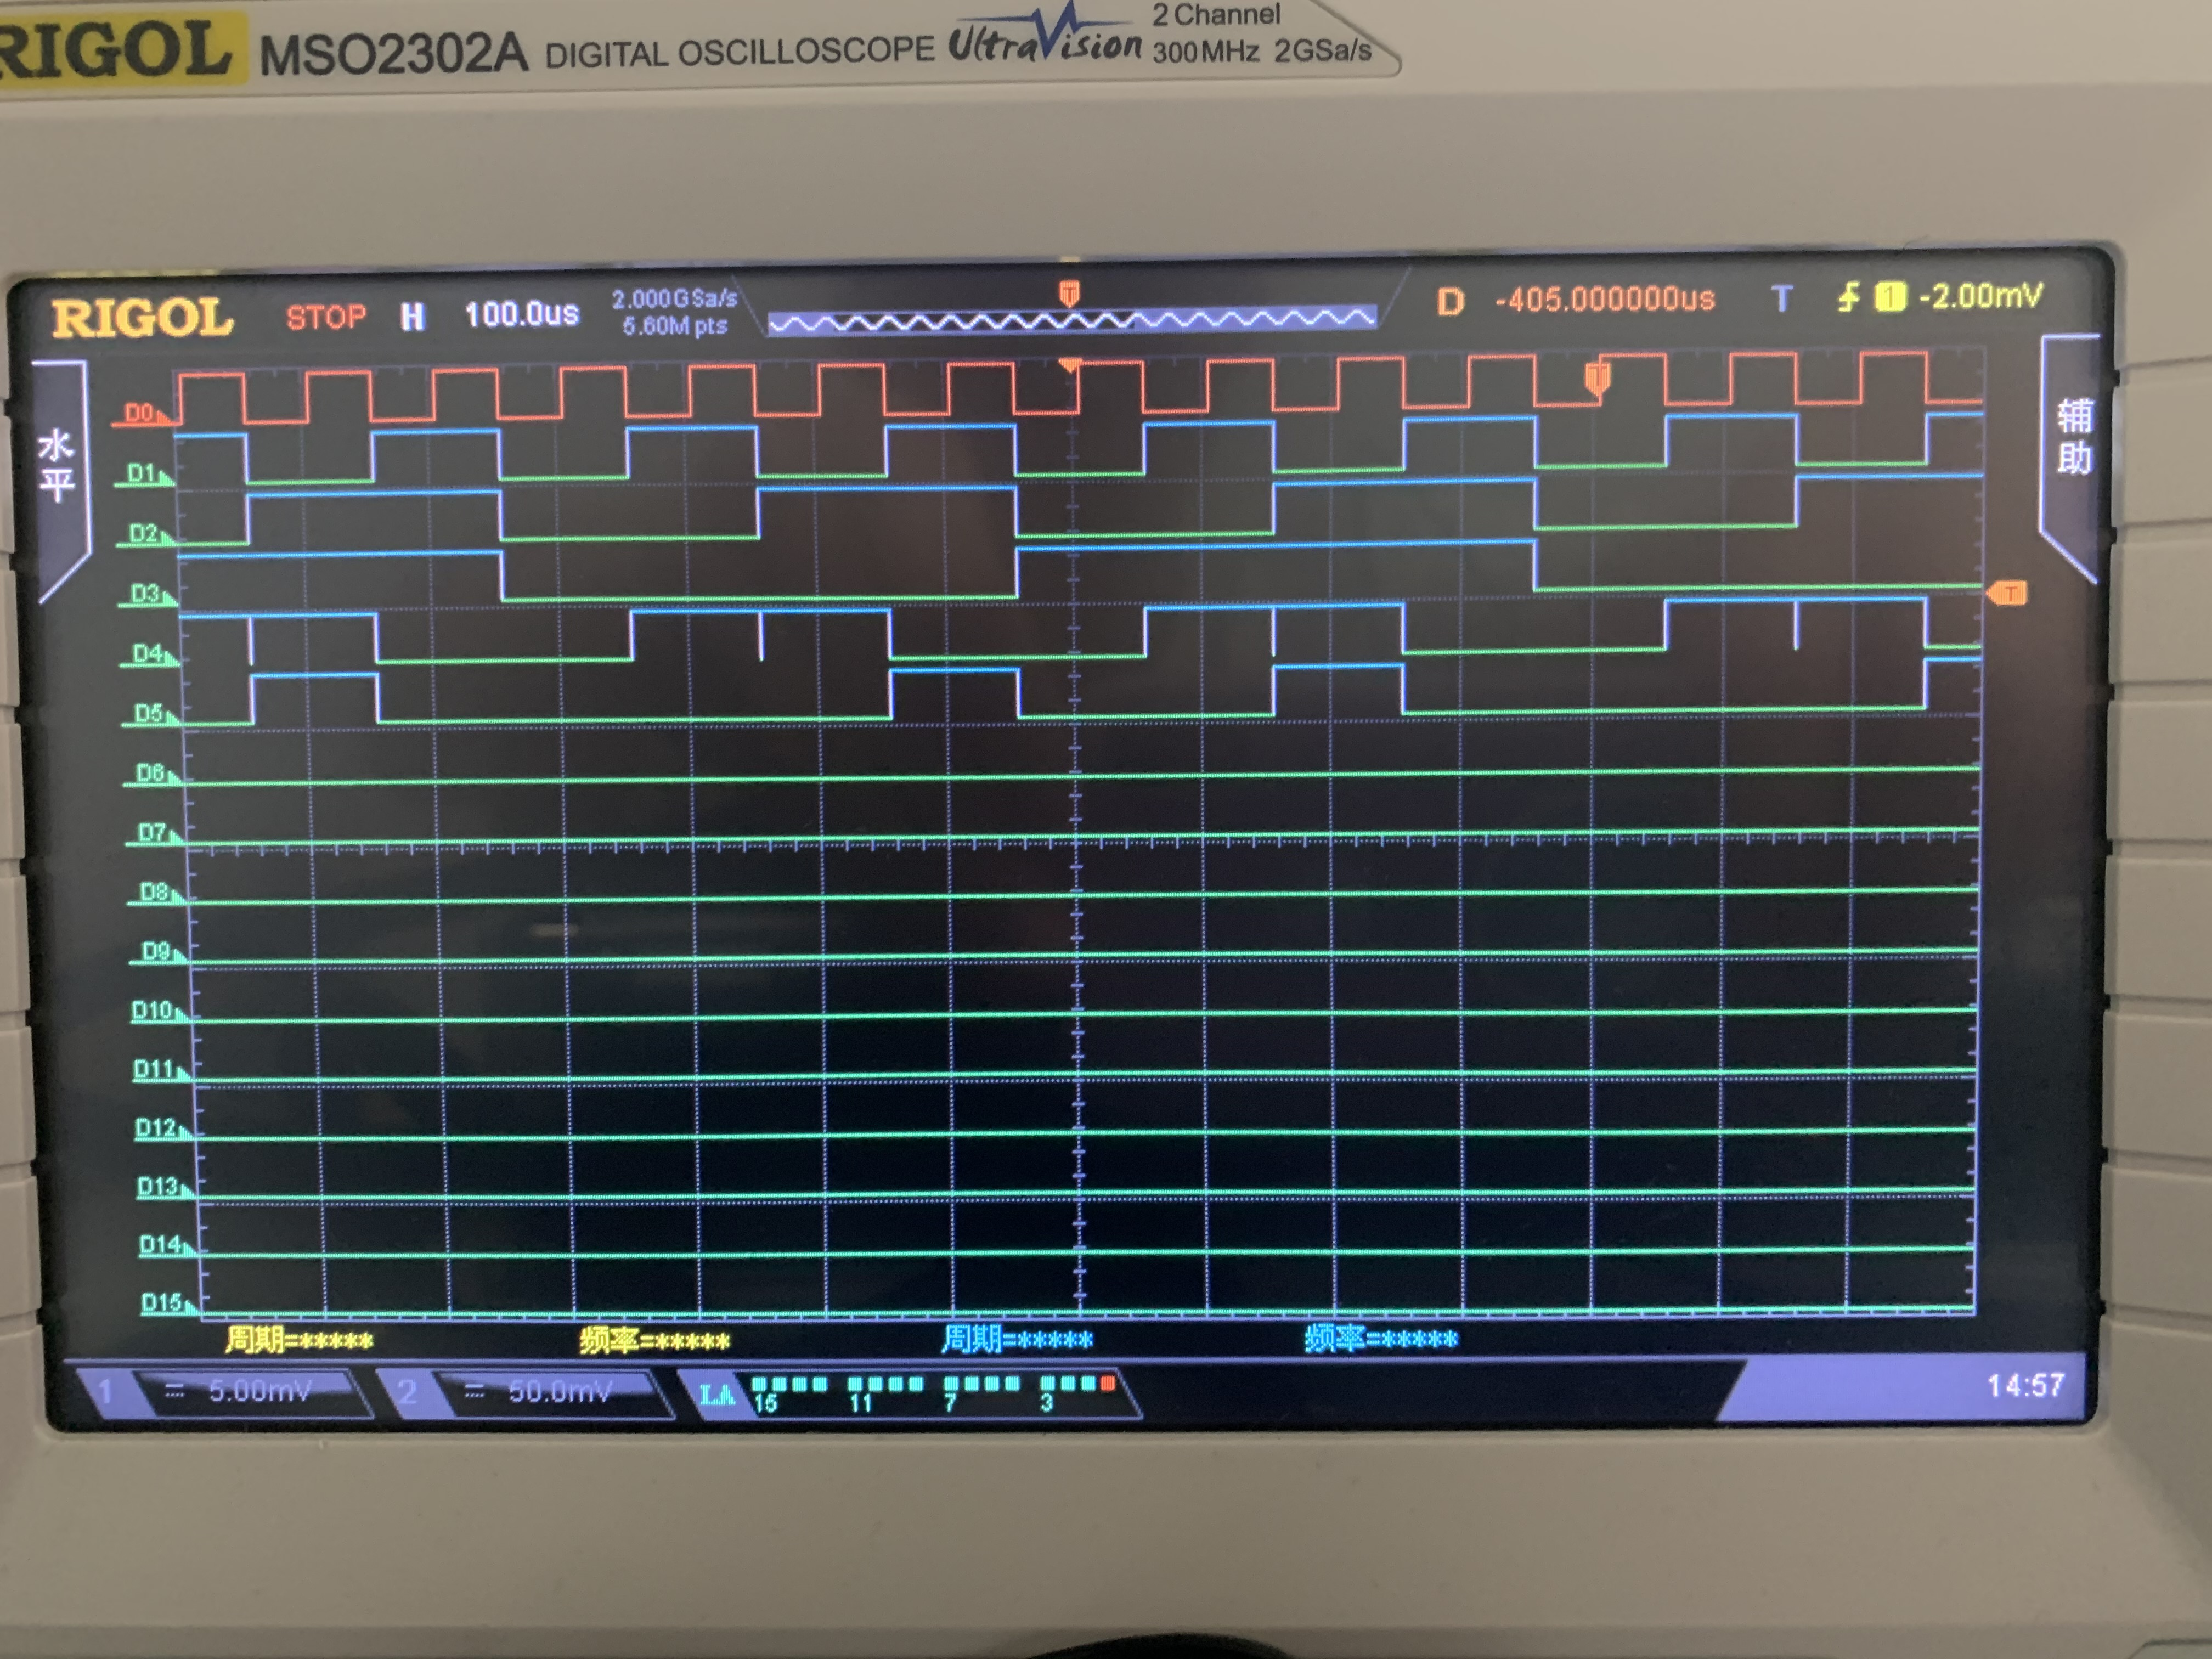
\includegraphics[width=0.8\textwidth]{AU.png}
\end{figure}
\subsection{LU}
\begin{figure}[H]
    \centering
    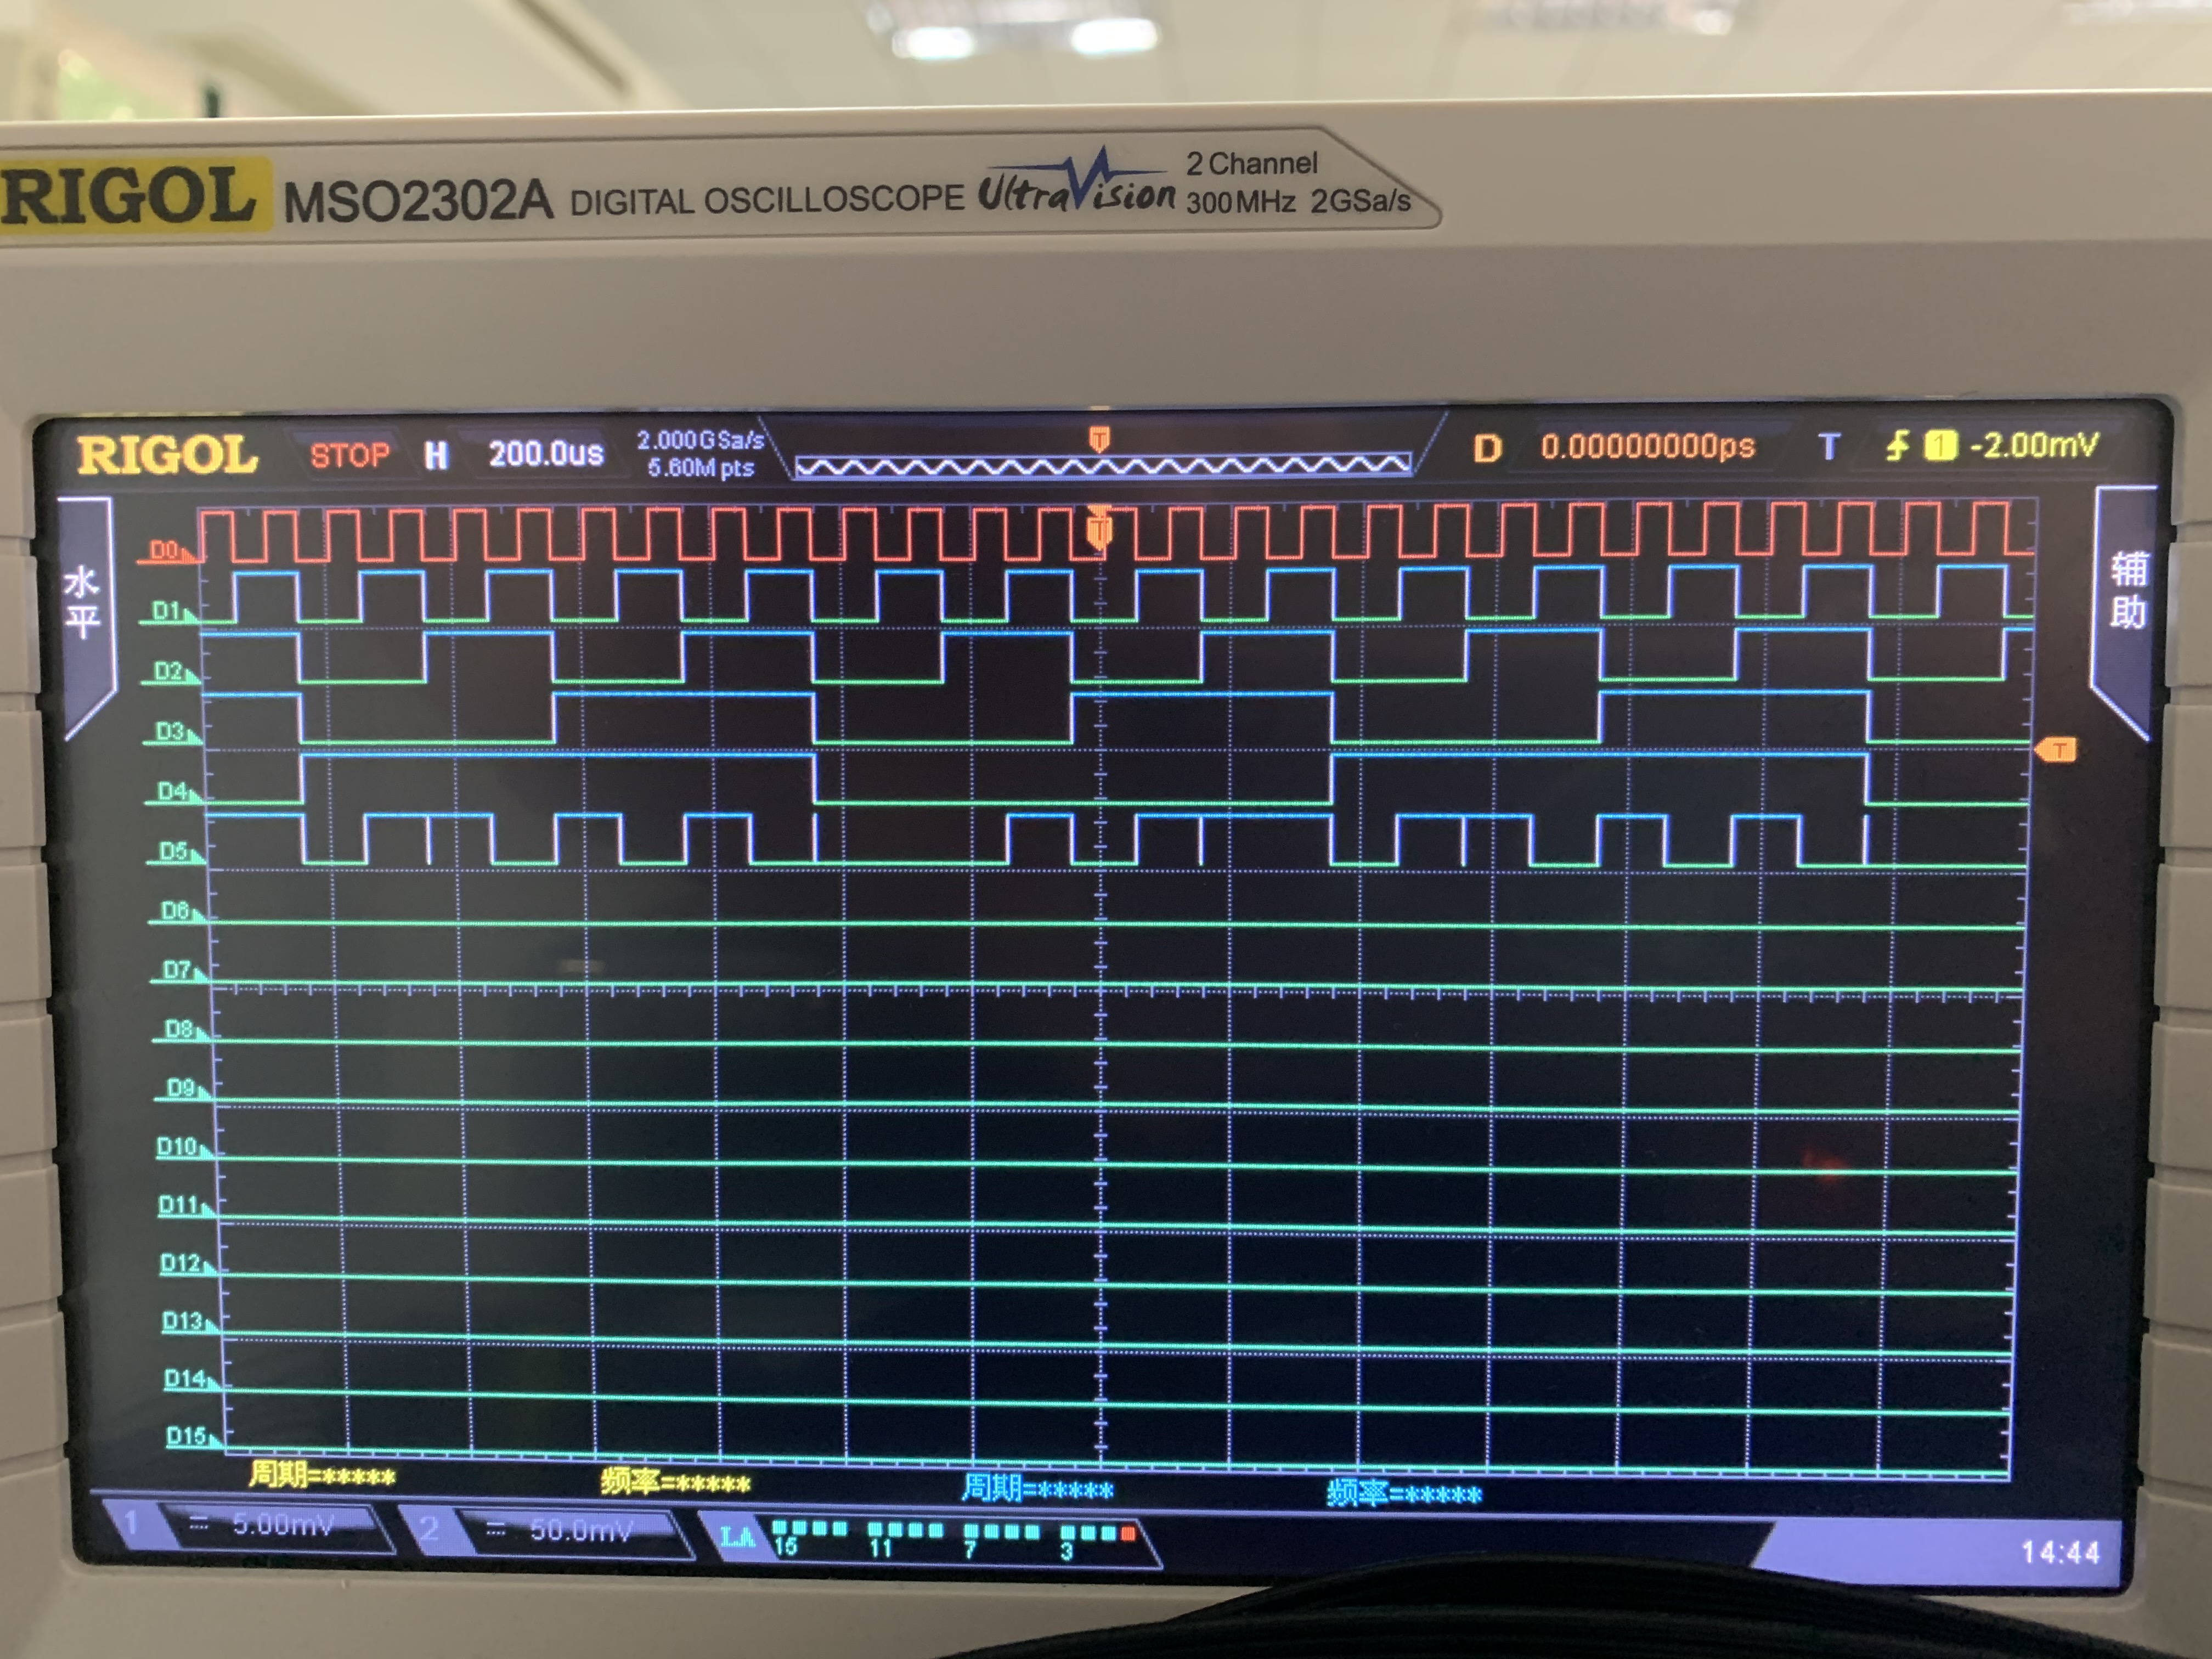
\includegraphics[width=0.8\textwidth]{LU.png}
\end{figure}
\section{实验总结}
学会使用选择器搭建一些电路。
%\clearpage
%\bibliography{E:/Papers/LiuLab}
%\bibliographystyle{apalike}
\end{document}
%%% Local Variables:
%%% mode: latex
%%% TeX-master: t
%%% End:
